\section{Wyrażenie regularne}

\subsection{Treść zadania}

\begin{figure}[h!]
    \centering
    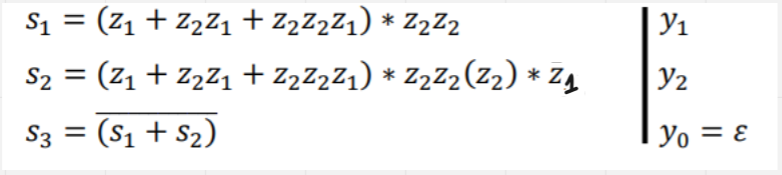
\includegraphics[width=.8\textwidth]{images/regex/reg_ex.png}
    \caption{treść zadania}
    \label{fig:my_label}
\end{figure}

Wyrażenia regularne to jeden wielki pierdolnik. Nasze wyrażenie podane w zadaniu podaje na wyjściu trzy możliwe wartości, $y_0$, $y_1$, $y_2$. $y_0$ pojawia się wtedy gdy nie jest aktywne ani $y_1$ ani $y_2$ xD. Opis całego wyrażenia sprowadza się do pracy nad $s_2$, bo w końcu $s_2$ zawiera w sobie $s_1$. Celem zadania jest skonstruowanie takiego układu czy narysowanie takiego grafu, który będzie się zachowywał dla odpowiednich wejść (z) tak jak jest to zapisane w wyrażeniu.

operatory używane w wyrażeniach regularnych:
\begin{itemize}
    \item Operator + oznacza sumę logiczną, czyli że w wyrażeniu możemy wybrać którą ścieżką pójdziemy np: $z_1$. + $z_2$. oznacza że możemy wybrać albo $z_1$ albo $z_2$. 
    \item Operator * oznacza iterację czyli że dana część ujęta w nawias przed gwiazdką może być wykonywana w nieskończoność (zero lub więcej razy).
\end{itemize}

\subsection{Czarna magia i techniki zakazane}

\subsubsection{Prolog}

\begin{figure}[h!]
    \centering
    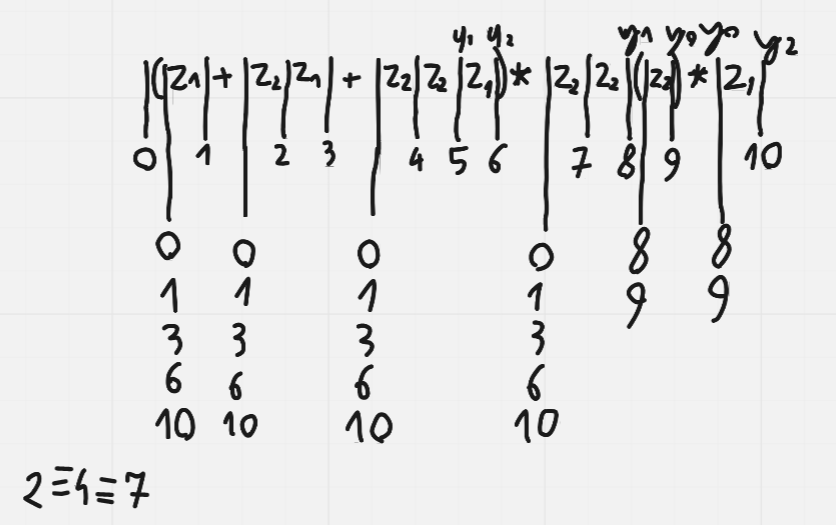
\includegraphics[width=.7\textwidth]{images/regex/reg_pp1.png}
    \caption{stany podstawowe i przedpodstawowe}
    \label{fig:my_label}
\end{figure}

\newpage

Tutaj zaczyna się dym. Stawiamy krótkie pionowe kreski po każdej zetce oraz na samym początku wyrażenia (tam oczywiście zapisujemy 0). Drugim krokiem jest narysowanie długich kresek na początku każdego słowa czyli przed dowolną grupką naszych $z_n$. Teraz trafiamy na jeden z bardziej problematycznych momentów, musimy ustalić do którego słowa można wejść z którego miejsca. Patrząc po rysunku, do słowa pierwszego w wyrażeniu czyli po prostu $z_1$ można wejść zera, ale można też do niego trafić gdy już przejdziemy przez wyraz $z_1$ czyli również z jedynki. Patrzymy dalej: jeśli przejdziemy przez słowo $z_2z_1$ możemy znowu przejść do słowa pierwszego (w naszym przypadku dalej $z_1$) czyli dopisujemy trójkę (bo nią kończy się słowo $z_2z_1$). To samo dla ostatniego słowa w iteracji. Ważnym jest że iterację można również ominąć, nikt ci nie każe wchodzić do pętli więc do pierwszego słowa za iteracją też można przejść z zera.
Jadąc do samego końca zauważamy, że z dziesiątki znowu można przejść na sam początek (zapętlamy działanie całego układu). Taka sytuacja z tego co zauważyliśmy ma miejsce tylko gdy wyrażenie zaczyna się od iteracji (tutaj jak ktoś wie coś więcej to prosimy o ekspertyzę). Patrząc na drugą iterację widzimy że do niej można przejść tylko z ósemki i dziewiątki. W końcu z samego początku żeby się tam dostać musimy przejść przez $z_2z_2$. Sporo tego a to dopiero początek xD. W lewym dolnym rogu mamy zapisane że 2 jest równoważna z czwórką i siódemką. Patrząc na wyrażenie widzimy że przejście do dwójki, czwórki i siódemki odbywa się poprzez przejście z 0,1,3,6,10 za pomocą $z_2$ czyli są one tożsame. Koniec kroku pierwszego. Xue hua piao piao.


\subsubsection{Niebagatelny zwrot akcji}

\begin{figure}[h!]
    \centering
    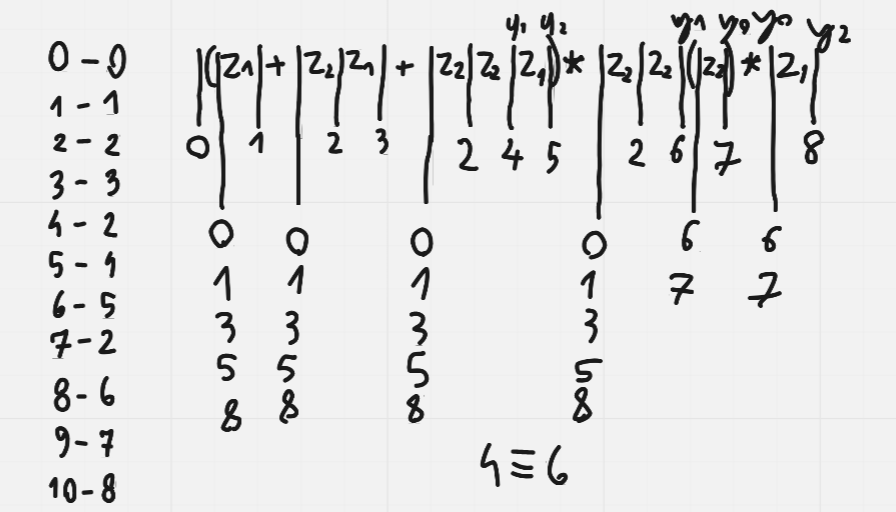
\includegraphics[width=.6\textwidth]{images/regex/reg_pp2.png}
    \caption{stany podstawowe i przedpodstawowe}
    \label{fig:my_label}
\end{figure}

Teraz będzie w miarę lekko, jako że $2\equiv4\equiv7$ to musimy trochę namieszać, rozpisujemy taką tabelkę jak po prawej stronie i widzimy, że: zero pozostało zerem, dwójka dwójką ale czwórka stała się dwójką. Skoro czwórka jest dwójką to tracimy jedną cyfrę, więc żeby zachować ciągłość przesuwamy wszystkie następne o jedną pozycję, czyli piątka staje się czwórką, szóstka piątką itd. Gdy dojdziemy do siódemki zapisujemy że jest ona równa dwójce, czyli oprócz tego że pozbyliśmy się czwórki to teraz nie ma jeszcze siódemki, czyli ósemka staje się szóstką.

Znowu patrzymy na nasze zmienione wyrażenie i widzimy że czwórka jest tożsama z szóstką, w końcu przejście do jednego i drugiego odbywa się poprzez dwójkę i $z_2$. No i proces powtarzamy do skutku aż już nic więcej nam się nie skróci.

\newpage

\subsubsection{Epilog}

\begin{figure}[h!]
    \centering
    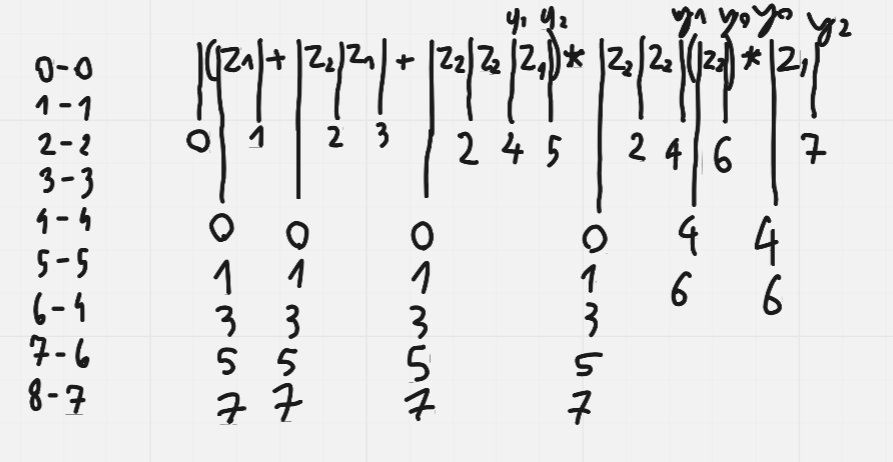
\includegraphics[width=.6\textwidth]{images/regex/reg_pp3.png}
    \caption{stany podstawowe i przedpodstawowe}
    \label{fig:my_label}
\end{figure}

Finalnie wyrażenie wygląda tak jak na obrazku. Jest trochę lepiej. Najtrudniejsze już za nami chociaż kolejny krok wymaga szczególnego skupienia bo łatwo o zasadzenie jakiegoś babola.

\subsection{Tabela stanów}

\begin{figure}[h!]
    \centering
    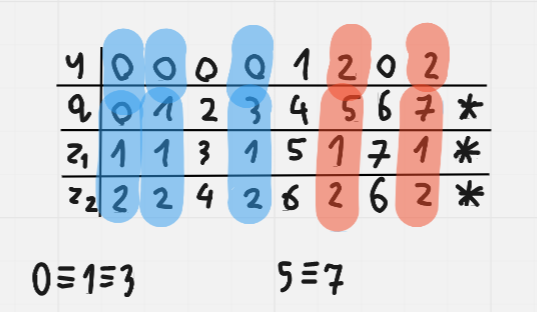
\includegraphics[width=.5\textwidth]{images/regex/reg_t1.png}
    \caption{tabela stanów}
    \label{fig:my_label}
\end{figure}

Jak widać na załączonym obrazku, stany $0\equiv1\equiv3$ oraz $5\equiv7$. 

Podczas minimalizowania stanów należy pamiętać o zgodności sygnałów wyjściowych. 

\newpage

\subsection{Zminimalizowana tabela stanów}

Po zminimalizowania tabeli, należy pamiętać o zmienieniu kolejności numerowania stanów.

\begin{figure}[h!]
    \centering
    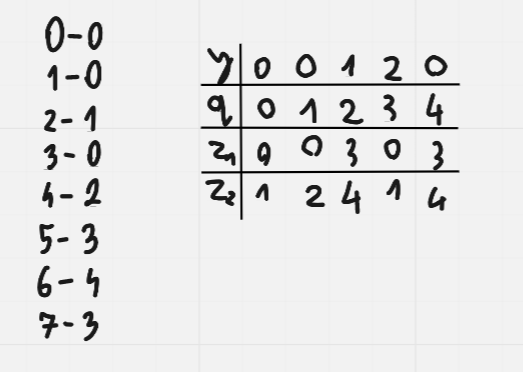
\includegraphics[width=.45\textwidth]{images/regex/reg_t2.png}
    \caption{zminimalizowana tabela stanów}
    \label{fig:my_label}
\end{figure}

\subsection{Finalny graf}

Na podstawie zminimalizowanej tabeli można w łatwy sposób (a jest w ogóle tutaj coś trudnego?) sporządzić końcowy graf ;)

\begin{figure}[h!]
    \centering
    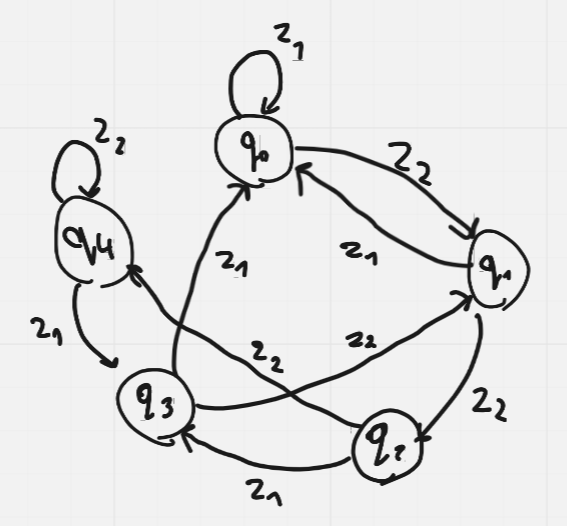
\includegraphics[width=.45\textwidth]{images/regex/reg_g.png}
    \caption{finalny graf}
    \label{fig:my_label}
\end{figure}

\subsection{Wyrażenie regularne grafu $G^{++}$}

Graf z poprzedniego podpunktu możemy również zapisać za pomocą oznaczeń. W tym celu rozpisujemy, w jakie miejsce przechodzi dany stan przy podaniu odpowiedniego wejścia:\\

$G^{++} = ^0(q_0^1(z_1q_0,z_2q_1^2(z_1q_0,z_2q_2^3(z_1q_3^4(z_1q_0,z_2q_1)^4,z_2q_4^4(z_1q_3,z_2q_4)^4)^3)^2)^1)^0$\\

Ten sam zapis, gotowy do skopiowania do programu (np. do statemachines czy APW):\\
$G^{++}$ = (q0(z1q0,z2q1(z1q0,z2q2(z1q3(z1q0,z2q1),z2q4(z1q3,z2q4)))))